\begin{note}
Presentation available on \url{https://guicho271828.github.io/2016-6-13-hsdip/} ; Press n/p key to move to next/previous slide
\end{note}

\begin{outline-text-1}
\begin{center}
Shoma Endo, \uline{Masataro Asai}, Alex Fukunaga

University of Tokyo
\end{center}
\end{outline-text-1}

\section{Satisficing Planning + Online Cost Refinements}
\label{sec-1}

\includegraphics{img/anytime1.png}

\section{Satisficing Planning + Algorithm Switch}
\label{sec-2}

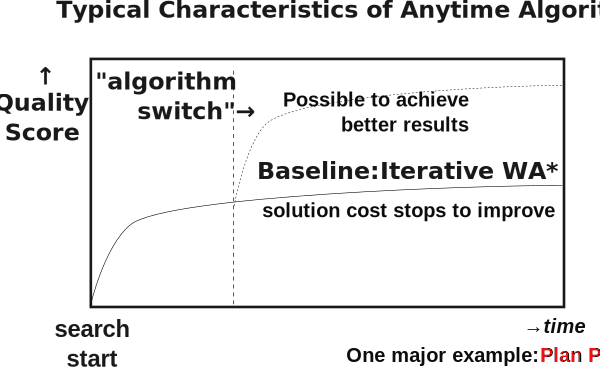
\includegraphics{img/anytime2.png}


\section{Main Topic of the paper: Plan Postprocessing}
\label{sec-3}

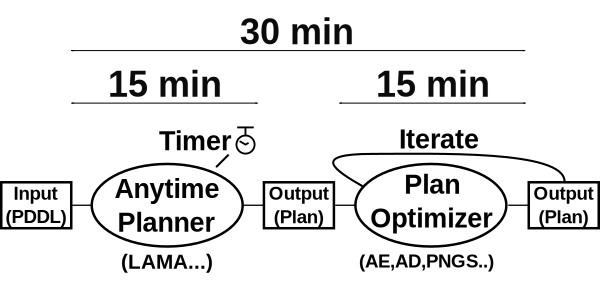
\includegraphics{img/framework.png}

\section{Various Postprocessing Systems}
\label{sec-4}

\begin{itemize}
\item Aras (Nakhost and Muller 2010)
\begin{itemize}
\item Action Elimination(\textbf{AE}) --- remove trivially redundant actions
\item Plan Neighborhood Graph Search(\textbf{PNGS}) --- replan on neighborhood graph
\end{itemize}
\item Action Dependency (\textbf{AD}) (Chrpa, McCluskey and Osborne 2012)
\begin{itemize}
\item Remove actions of inverse effects etc.
\end{itemize}
\item Block Deordering (BDPO2) (Siddiqui and Haslum 2013;2015)
\begin{itemize}
\item convert the input to partial order blocks, replan each block
\end{itemize}
\item Anytime Iterative Refinement of Solution (\textbf{AIRS}) (Estrem and Krebsbach 2012)
\end{itemize}

\section{Two groups of Optimization Algorithms}
\label{sec-5}

\begin{center}
\begin{tabular}{clc}
Polytime Optimizer &  & Search-based Optimizer\\
\hline
Based on the direct &  & External solver refines\\
analysis of a given plan &  & a partial segment in a plan\\
\hline
 &  & \\
 &  & \\
 &  & \\
\hline
\end{tabular}
\end{center}

\subsection{Polytime Optimizers}
\label{sec-5-1}

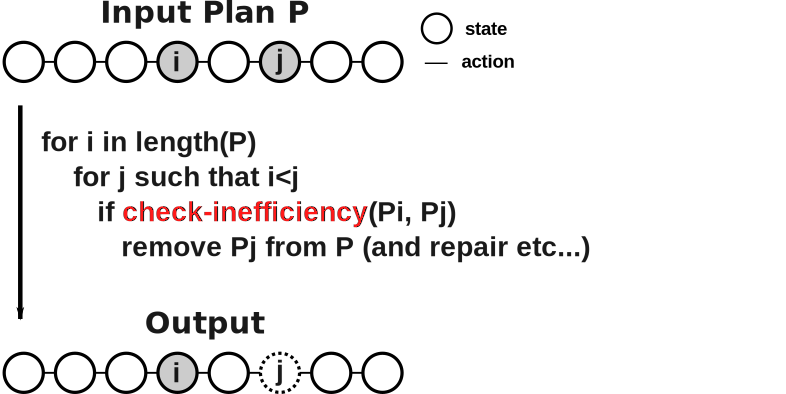
\includegraphics{img/polytime.png}

\subsection{Polytime Optimizers}
\label{sec-5-2}

\includegraphics{img/polytime2.png}

\subsection{Two groups of Optimization Algorithms}
\label{sec-5-3}

\begin{center}
\begin{tabular}{clc}
Polytime Optimizer &  & Search-based Optimizer\\
\hline
Based on the direct &  & External solver refines\\
analysis of a given plan &  & a partial segment in a plan\\
\hline
\textbf{AE : O(n$^{\text{2}}$)} &  & \\
\textbf{AD : O(n$^{\text{2}}$)} &  & \\
n: plan length &  & \\
\hline
\end{tabular}
\end{center}

\subsection{Search-based Optimizers}
\label{sec-5-4}

\includegraphics{img/search-based.png}

\subsection{Search-based Optimizers}
\label{sec-5-5}

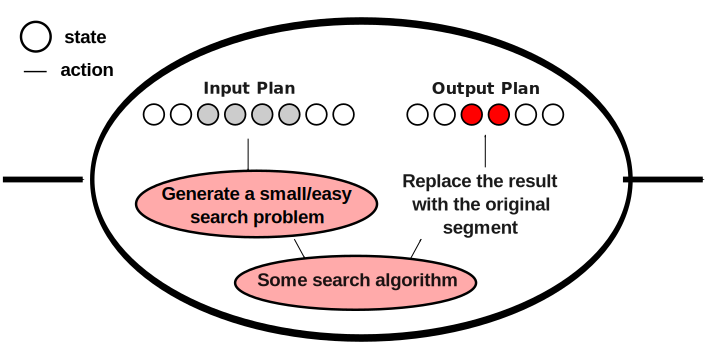
\includegraphics{img/search-based2.png}

\subsection{Two groups of Optimization Algorithms}
\label{sec-5-6}

\begin{center}
\begin{tabular}{clc}
Polytime Optimizer &  & Search-based Optimizer\\
\hline
Based on the direct &  & External solver refines\\
analysis of a given plan &  & a partial segment in a plan\\
\hline
AE : O(n$^{\text{2}}$) &  & \textbf{PNGS}\\
AD : O(n$^{\text{2}}$) &  & \textbf{AIRS}\\
n: plan length &  & BDPO2\\
\hline
\end{tabular}
\end{center}

\subsection{Search-based Optimizers Taxonomy}
\label{sec-5-7}

\begin{container-fluid}
\begin{row-fluid}
\begin{span3}


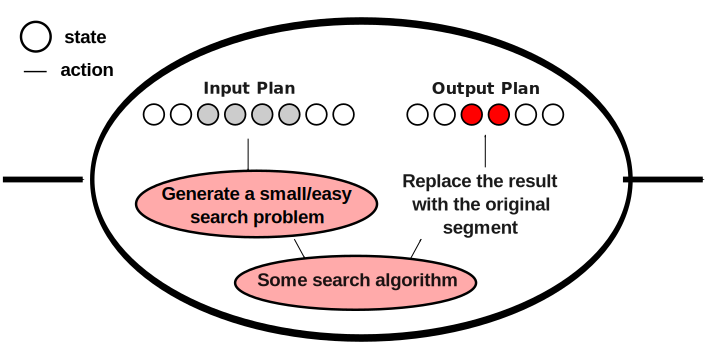
\includegraphics{img/search-based2.png}
\end{span3}
\begin{span9}
\begin{center}
\begin{tabular}{lll}
 & Subproblems Generation & Underlying Solver\\
\hline
PNGS & neighborhood graph & \\
 & (search space around the plan) & \\
AIRS & windows (ordered by Δcost/Δh) & \\
BDPO2 & windows (block decomposition) & \\
 &  & \\
\end{tabular}
\end{center}
\end{span9}
\end{row-fluid}
\end{container-fluid}

\subsection{Window-based optimization}
\label{sec-5-8}

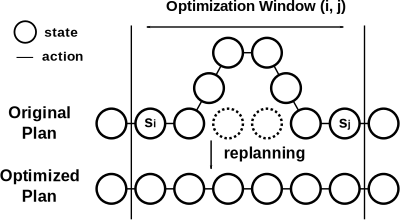
\includegraphics{img/window.png}

\subsection{Search-based Optimizers Taxonomy}
\label{sec-5-9}

\begin{container-fluid}
\begin{row-fluid}
\begin{span2}


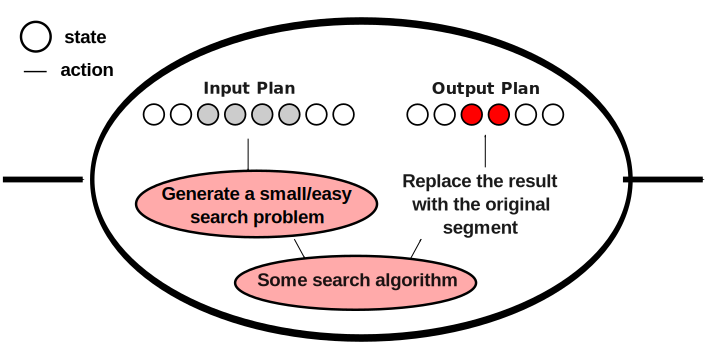
\includegraphics{img/search-based2.png}
\end{span2}
\begin{span10}
\begin{center}
\begin{tabular}{lll}
 & Subproblems Generation & Underlying Solver\\
\hline
PNGS & neighborhood graph & Blind unit-cost A*\\
 & (search space around the plan) & or Backward Breadths First\\
AIRS & windows (ordered by Δcost/Δh) & Blind Bidirectional\\
BDPO2 & windows (block decomposition) & Admissible A*\\
 &  & or PNGS (layered approach)\\
\end{tabular}
\end{center}
\end{span10}
\end{row-fluid}
\end{container-fluid}


\section{Open Questions}
\label{sec-6}

\begin{larger}
\textbf{What is the \emph{baseline} of various search-based optimizers?}
\end{larger}

\begin{alignright}
i.e. Are these \textbf{\emph{complex}} algorithms necessary?
\end{alignright}

 

\begin{larger}
\textbf{How to \emph{combine} Polytime and Search-based Optimizers?}
\end{larger}

\begin{alignright}
Also, how effective is it to combine them?
\end{alignright}

\section{Various Minor Differences in Search-based Optimizers ☹}
\label{sec-7}

\begin{center}
\begin{tabular}{lll}
 & Subproblems Generation & Underlying Solver\\
\hline
PNGS & \textbf{neighborhood graph} & \textbf{Blind} unit-cost A*\\
 & (search space around the plan) & or \textbf{Backward Breadths First}\\
AIRS & windows \textbf{(ordered by Δcost/Δh)} & \textbf{Blind Bidirectional}\\
BDPO2 & windows \textbf{(block deordering)} & Admissible A*\\
 &  & or \textbf{PNGS} (layered approach)\\
\hline
 &  & \\
\end{tabular}
\end{center}

\begin{alignright}
\begin{larger}
\textbf{→ Hard to obtain a useful observation from the experiments}
\end{larger}
\end{alignright}

\section{\emph{Simplest baseline} of search-based optimizers : \textbf{\emph{R-WIN}}}
\label{sec-8}

\begin{center}
\begin{tabular}{lll}
 & Subproblems Generation & Underlying Solver\\
\hline
PNGS & neighborhood graph & Blind unit-cost A*\\
 & (search space around the plan) & or Backward Breadths First\\
AIRS & windows (ordered by Δcost/Δh) & Blind Bidirectional\\
BDPO2 & windows (block deordering) & Admissible A*\\
 &  & or PNGS (layered approach)\\
\hline
\textbf{\emph{R-WIN}} & \textbf{windows} (\textbf{random}) & \textbf{Admissible A$^{\text{*}}$ + LMcut}\\
\end{tabular}
\end{center}

\section{Evaluate them in an "\emph{Equal Condition}"}
\label{sec-9}

\begin{center}
\begin{tabular}{lll}
 & Subproblems Generation & Underlying Solver\\
\hline
PNGS & neighborhood graph & \textbf{Admissible A$^{\text{*}}$ + LMcut}\\
 & (search space around the plan) & \\
AIRS & windows (ordered by Δcost/Δh) & \textbf{Admissible A$^{\text{*}}$ + LMcut}\\
BDPO2 & windows (block deordering) & \textbf{Admissible A$^{\text{*}}$ + LMcut}\\
 &  & \\
\hline
R-WIN & windows (random) & \textbf{Admissible A$^{\text{*}}$ + LMcut}\\
\end{tabular}
\end{center}

\begin{alignright}
\begin{larger}
\textbf{→ Focus on the subproblem generation}
\end{larger}
\end{alignright}

\section{Evaluation}
\label{sec-10}

\begin{container-fluid}
\begin{row-fluid}
\begin{span6}
39 IPC domains

Optimize the 15 min, 2GB results of LAMA

Resource 15 min, 2GB

Participants AD, AE, AIRS, PNGS, R-WIN

(BDPO2 is not tested)

(AD, AE as a point of reference)
\end{span6}
\begin{span6}
\begin{center}
\begin{tabular}{lr}
Algorithm & Harmonic Means\\
 & of Ratios\\
\hline
LAMA(15min) & 100\%\\
LAMA(30min) & \%\\
AE & \%\\
AD & \%\\
AIRS & \%\\
PNGS & \%\\
R-WIN & \%\\
\end{tabular}
\end{center}
\end{span6}
\end{row-fluid}
\end{container-fluid}

\begin{alignright}
 
\end{alignright}

\section{Results}
\label{sec-11}

\begin{container-fluid}
\begin{row-fluid}
\begin{span6}
39 IPC domains

Optimize the 15 min, 2GB results of LAMA

Resource 15 min, 2GB

Participants AD, AE, AIRS, PNGS, R-WIN

(BDPO2 is not tested)

(AD, AE as a point of reference)
\end{span6}
\begin{span6}
\begin{center}
\begin{tabular}{ll}
Algorithm & Harmonic Means\\
 & of Ratios\\
\hline
LAMA(15min) & 100\%\\
LAMA(30min) & 99.3\%\\
AE & 98.4\%\\
AD & 97.4\%\\
AIRS & 97.9\%\\
PNGS & 96.0\%\\
R-WIN & \textbf{95.9\%}\\
\end{tabular}
\end{center}
\end{span6}
\end{row-fluid}
\end{container-fluid}

\begin{alignright}
\begin{larger}
\textbf{Complex tweaks did not outperform the simplest variant}
\end{larger}
\end{alignright}

\section{}
\label{sec-12}

\begin{xlarge}
\begin{center}
☹

Sadly "Improvements" did not outperform the simplest baseline
\end{center}
\end{xlarge}

\section{}
\label{sec-13}

\begin{xlarge}
\begin{center}
☺

Luckily we have a reliable baseline to improve upon!
\end{center}
\end{xlarge}

\section{Improve AIRS to outperform R-WIN: \textbf{\emph{CH-WIN}}}
\label{sec-14}

\begin{larger}
Why we chose AIRS?

\begin{alignright}
→ \textbf{Easy} to implement, \textbf{minimum diff} from R-WIN
\end{alignright}

Problem in AIRS:

\begin{center}
Original AIRS is tested only on
\end{center}

\begin{alignright}
\textbf{small-scale 15-puzzle/grid-pathfinding}

\textbf{< 0.1 sec replanning time}
\end{alignright}
\end{larger}

\section{Window Priority Scheme in AIRS}
\label{sec-15}

\begin{larger}
Priority: \textbf{Δcost(i,j) / Δh(i,j)}
\end{larger}

\includegraphics{img/airs.png}

\begin{alignright}
\begin{larger}
Priority seems promising, \textbf{but\ldots{}}
\end{larger}
\end{alignright}

\section{AIRS Pitfall 1 : Windows may be too long/difficult}
\label{sec-16}

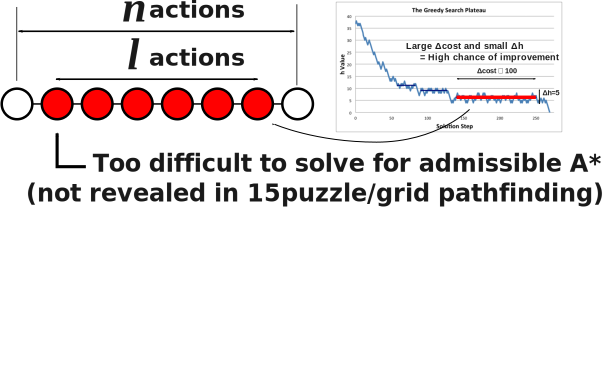
\includegraphics{img/binary-search.png}

\subsection{AIRS Pitfall 1 : Windows may be too long/difficult}
\label{sec-16-1}

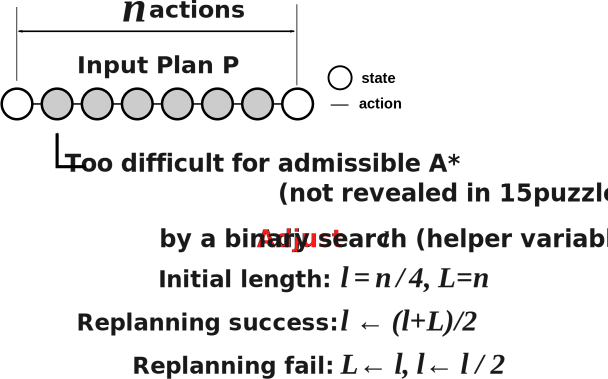
\includegraphics{img/binary-search2.png}

\section{AIRS Pitfall 2 : Inappropriate Penalty Scheme}
\label{sec-17}

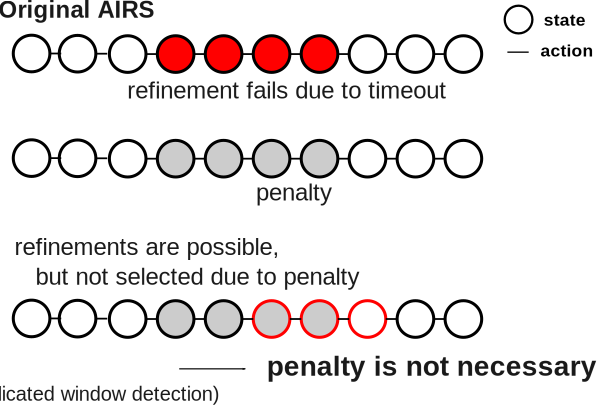
\includegraphics{img/penalty.png}

\subsection{AIRS Pitfall 2 : Inappropriate Penalty Scheme}
\label{sec-17-1}

\includegraphics{img/penalty2.png}

\section{AIRS Pitfall 3 : Overly Complicated → Keep it simple}
\label{sec-18}

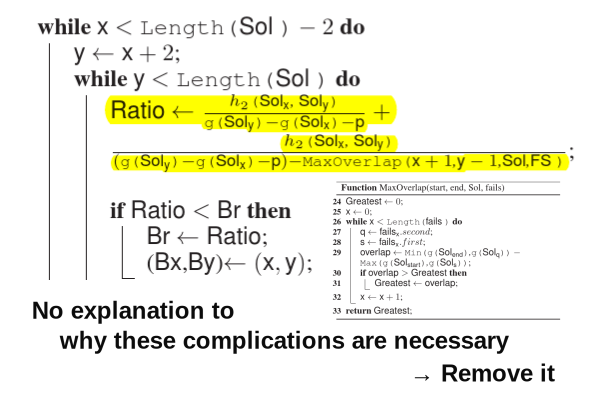
\includegraphics{img/toocomplicated.png}

\section{Result}
\label{sec-19}

\begin{larger}
CH-WIN achieved the \textbf{best performance}
\end{larger}

\begin{center}
\begin{tabular}{ll}
Algorithm & Harmonic Means\\
 & of Ratios\\
\hline
LAMA(15min) & 100\%\\
LAMA(30min) & 99.3\%\\
AE & 98.4\%\\
AD & 97.4\%\\
AIRS & 97.9\%\\
PNGS & 96.0\%\\
R-WIN & 95.9\%\\
\hline
\textbf{CH-WIN (proposed)} & \textbf{93.3\%}\\
\end{tabular}
\end{center}

\section{Open Questions}
\label{sec-20}

\begin{larger}
\sout{What is the \emph{baseline} of various search-based optimizers?}
\end{larger}

\begin{alignright}
\sout{i.e. Are these \textbf{\emph{complex}} algorithms necessary?} → Simple algorithms perform better
\end{alignright}

 

\begin{larger}
\textbf{How to \emph{combine} Polytime and Search-based Optimizers?}
\end{larger}

\begin{alignright}
Also, how effective is it to combine them?
\end{alignright}

\section{Multiple Optimizers}
\label{sec-21}

\includegraphics{img/framework2.png}

\subsection{Multiple Optimizers}
\label{sec-21-1}

\includegraphics{img/framework3.png}

\subsection{Iterating Polytime Optimizer}
\label{sec-21-2}

\includegraphics{img/static/poly.png}

\begin{alignright}
\begin{larger}
\begin{itemize}
\item Iterating AE and AD is not effective
\item we can safely assume that we apply them \textbf{at most once}
\end{itemize}
\end{larger}
\end{alignright}

\section{Polytime + Search-based Result}
\label{sec-22}

\begin{center}
\begin{tabular}{l|r|r|}
Algorithm &  & \\
\emph{x} & \emph{x} only & AE+AD+ \emph{x}\\
\hline
LAMA(15min) & 100\% & -\\
LAMA(30min) & 99.3\% & -\\
AE & 97.4\% & \\
AD & 98.4\% & \\
AIRS & 97.9\% & 95.6\%\\
PNGS & 96.0\% & 94.4\%\\
R-WIN & 95.9\% & 94.0\%\\
\hline
\textbf{CH-WIN (proposed)} & 93.3\% & \textbf{91.8\%}\\
\end{tabular}
\end{center}

\section{Lessons Learned}
\label{sec-23}

\begin{itemize}
\item \textbf{Avoid} unnecessary complexity
\item \textbf{R-WIN}, baseline, outperformed AIRS, PNGS etc.
\begin{itemize}
\item Use the simplest variant as a baseline, improve upon it
\end{itemize}
\item CH-WIN, an improved AIRS variant, outperformed previous algorithms
\item Reconfirmed poly+search effectiveness
\end{itemize}

\begin{center}
\begin{larger}
Thank you for Listening!
\end{larger}
\end{center}
